\documentclass[../masters.tex]{subfiles}

\begin{document}
\graphicspath{{./imgs/}{../imgs/}} %look for images

\section{Nonlinear Models}
In this section we still consider probabilistic graphical models of the form shown in Figure \ref{fig_linmod}. The variables retain their meaning as before but we generalise the model by dropping the linearity assumption. Unfortunately, this generalisation, although allowing us to expand our investigation to a much more expressive class of models, makes closed form solutions to the inference problem intractable in general.   
\begin{figure}[H] 
\centering
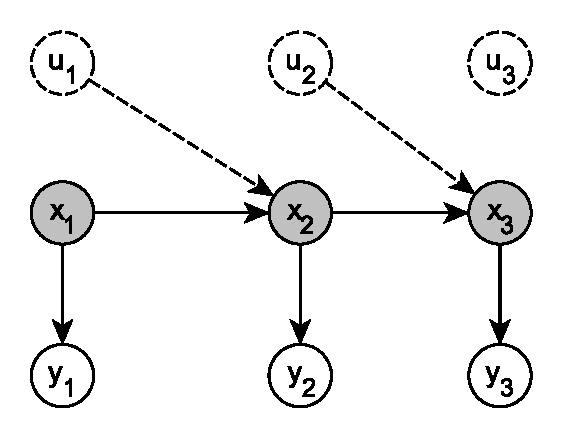
\includegraphics[scale=1.0]{linear_model.pdf}
\caption{Graphical model of this section}
\label{fig_linmod}
\end{figure}
We again assume that the transition and emission functions are time invariant. The state space model is now of the form (\ref{eq_statespace}).
\begin{equation}
\begin{aligned}
x_{t+1} &= f(x_t, u_t, w_{t+1}) \\
y_{t+1} &= g(x_{t+1}, v_{t+1})
\end{aligned}
\label{eq_statespace}
\end{equation}
Note that we make no assumption about the functional form of the noise terms $w_t,v_t$. In practice it is customary to assume that they have zero mean but otherwise are not restricted.

\subsection{Sequential Monte Carlo Methods}
Many approximate inference techniques exist in literature but we shall focus only on Sequential Monte Carlo (SMC) methods because it is simple to implement and generalises well (and easily) to more complex graphical models. 

SMC methods are a general class of Monte Carlo methods which sample sequentially from the growing target distribution $\pi_t(x_{1:t})$. By only requiring that $\gamma_t$ be known point-wise we have the framework of SMC methods as shown in (\ref{eq_SMC1}). Note that $Z_t$ is some normalisation constant \cite{pftut}.
\begin{equation}
\begin{aligned}
\pi_t(x_{1:t}) &= \frac{\gamma_t(x_{1:t})}{Z_t} \\
Z_t &= \int_{x_{1:t}} \gamma_t(x_{1:t})
\end{aligned}
\label{eq_SMC1}
\end{equation} 
For example, in the context of filtering we have that $\gamma_t(x_{1:t}) = p(x_{1:t},y_{1:t})$ and $Z_t = p(y_{1:t})$ so that $\pi_t(x_{1:t}) = p(x_{1:t}|y_{1:t})$. 

It is possible to approximate the distribution $\pi_t(x_{1:t})$ by drawing $N$ samples $X_{1:t}^i \backsim \pi_t(x_{1:t})$ and using the Monte Carlo method to find the approximation $\hat{\pi}_t(x_{1:t})$ as shown in (\ref{eq_SMC2}).
\begin{equation}
\hat{\pi}_t(x_{1:t}) = \frac{1}{N}\sum_{i=1}^N \delta(X^i_{1:t}, x_{1:t})
\label{eq_SMC2}
\end{equation}
We denote the Dirac Delta function of $x$ with mass located at $x_0$ by $\delta(x_0,x)$. It is easy to approximate the marginal $\pi_t(x_{t})$ as shown in (\ref{eq_SMC3}).
\begin{equation}
\hat{\pi}_t(x_{t}) = \frac{1}{N}\sum_{i=1}^N \delta(X^i_{t}, x_{t})
\label{eq_SMC3}
\end{equation}
It can be shown that the variance of the approximation error of $\pi_t$ decreases at rate $\mathcal{O}(\frac{1}{N})$. Unfortunately there are two significant drawbacks to the Monte Carlo approximation. The first is that often we cannot sample from $\pi_t(x_{1:t})$ directly and the second is that even if we could it is often computationally prohibitive. 

We use the Importance Sampling method to address the first problem. We do this by introducing an importance (sometimes called proposal) density $q_t(x_{1:t})$ such that $\pi_t(x_{1:t}) > 0 \implies q_t(x_{1:t}) > 0$. By substituting this into the SMC framework (\ref{eq_SMC1}) we have (\ref{eq_SMC4}).
\begin{equation}
\begin{aligned}
\pi_t(x_{1:t}) &= \frac{w_t(x_{1:t})q_t(x_{1:t})}{Z_t} \\
Z_t &= \int_{x_{1:t}} w_t(x_{1:t})q_t(x_{1:t})
\end{aligned}
\label{eq_SMC4}
\end{equation} 
Where we have defined the unnormalised weight function $w_t(x_{1:t}) = \frac{\gamma_t(x_{1:t})}{q_t(x_{1:t})}$. It is possible, for example, to set $q_t$ to a multivariate Gaussian which is easy to sample from. By drawing $N$ samples $X_{1:t}^i \backsim q_t(x_{1:t})$ and using (\ref{eq_SMC4}) we have (\ref{eq_SMC5}). 
\begin{equation}
\begin{aligned}
\hat{\pi}_t(x_{1:t}) &= \frac{1}{N}\sum_{i=1}^N W_t^i\delta(X^i_{1:t}, x_{1:t}) \\
\hat{Z}_t &= \frac{1}{N}\sum_{i=1}^N w_t(X^i_{1:t}) \\
W^i_t &= \frac{w_t(X^i_{1:t})}{\sum_{i=1}^N w_t(X^i_{1:t})}
\end{aligned}
\label{eq_SMC5}
\end{equation}
Now we will attempt to modify the Importance Sampling method to address the second problem of computational cost incurred by the sampling routine. 

We do this by selecting an importance/proposal distribution which factorises according to $q_t(x_{1:t}) = q_{t-1}(x_{1:t-1})q_t(x_{t}|x_{1:t-1}) = q_1(x_1) \Pi_{k=2}^t q_k(x_k|x_{1:k-1})$. In this way we only need to sample sequentially at each time step: at time $t=1$ we sample $X_1^i \backsim q_1(x_1)$, at time $t=2$ we sample $X_{2}^i \backsim q_2(x_2|x_1)$ and so we build up $X^i_{1:t} \backsim q_t(x_{1:t})$ factor by factor.

The weights can be written in the form (\ref{eq_SMC6}).
\begin{equation}
\begin{aligned}
w_t(x_{1:t}) &= \frac{\gamma_t(x_{1:t})}{q_t(x_{1:t})} \\
&= \frac{\gamma_{t-1}(x_{1:t-1})}{q_{t-1}(x_{1:t-1})}\frac{\gamma_t(x_{1:t})}{\gamma_{t-1}(x_{1:t-1})q_t(x_t|x_{1:t-1})} \\
&= w_{t-1}(x_{1:t-1})\alpha_t(x_{1:t-1}) \\
&= w_1(x_1)\Pi_{k=2}^t \alpha_k(x_{1:k})
\end{aligned}
\label{eq_SMC6}
\end{equation}
Thus, at any time $t$ we can obtain the estimates $\hat{\pi}_t(x_{1:t})$ and $Z_t$. The major limitation of this approach is that the variance of the resulting estimates typically increases exponentially with $t$ \cite{pftut}. 

We overcome this problem by resampling and thus introduce the Sequential Importance Resampling (SIR) method. So far we have a set of weighted samples generated from $q_t(x_{1:t})$ which builds the approximation $\hat{\pi}_t(x_{1:t})$. However, sampling directly from $\hat{\pi}_t(x_{1:t})$ does not approximate $\pi_t(x_{1:t})$. To obtain an approximate distribution of $\pi_t(x_{1:t})$ we need to sample from the weighted distribution $\hat{\pi}_t(x_{1:t})$. This is called resampling because we are sampling from a sampled distribution. Many techniques exist to perform this step efficiently. The crudest and most widely used one is to simply use the discrete multinomial distribution based on $W^i_{1:t}$ to draw samples from $\hat{\pi}_t(x_{1:t})$ \cite{pftut}. 

The benefit of resampling is that it allows us to remove particles with low weight and thus keeps the variance of the estimate in check. We are finally ready to consider the general SIR  algorithm:

For $t=1$:
\begin{enumerate}
\item
Sample $X^i_1 \backsim q_1(x_1)$.
\item
Compute the weights $w_1(X_1)$ and $W^i_1 \propto w_1(X^i_1)$.
\item
Resample $(W^i_1, X^i_1)$ to obtain $N$ equally weighted particles $(\frac{1}{N}, \bar{X}^i_1)$.
\end{enumerate}
For $t \geq 2$:
\begin{enumerate}
\item
Sample $X^i_t \backsim q_t(x_t|\bar{X}^i_{1:t-1})$ and set ${X}^i_{1:t} \leftarrow (\bar{X}^i_{1:t-1}, X^i_t)$ .
\item
Compute the weights $\alpha_t(X^i_{1:t})$ and $W^i_t \propto \alpha_t(X^i_{1:t})$.
\item
Resample $(W^i_t, X^i_{1:t})$ to obtain $N$ equally weighted particles $(\frac{1}{N}, \bar{X}^i_{1:t})$.
\end{enumerate}
At any time $t$ we have two approximations for $\pi(x_{1:t})$ as shown in (\ref{eq_smc_algo}).
\begin{equation}
\begin{aligned}
\hat{\pi}(x_{1:t}) &= \sum_{i=1}^N W^i_t \delta(X^i_{1:t}, x_{1:t}) \\
\bar{\pi}(x_{1:t}) &= \frac{1}{N}\sum_{i=1}^N \delta(\bar{X}^i_{1:t}, x_{1:t})
\end{aligned}
\label{eq_smc_algo}
\end{equation}
The latter approximation represents the resampled estimate and the former represents the sampled estimate \cite{pftut}. We prefer the former because in the limit as $N \rightarrow \infty$ it is a better approximation of $\pi_t$. However, as we have mentioned the variance of $\hat{\pi}(x_{1:t})$ tends to be unbounded and thus we often have that most of the particles in the particle population have very low weight. From a computational point of view this is wasteful. To ameliorate this we use the latter, resampled, estimate. However, the problem with the resampled estimate is that it effectively culls low weight particles and this reduces the diversity of the particle population \cite{murphy1}. 

We attempt to get the benefit of both worlds by only performing resampling when the weight variance of the particles becomes large. The Effective Sample Size (ESS) is a method whereby one determines when to perform resampling according to (\ref{eq_ess}).
\begin{equation}
\text{ESS} = \frac{1}{\sum_{i=1}^N (W^i_n)^2}
\label{eq_ess}
\end{equation} 
If the ESS becomes smaller than some threshold (typically $\frac{N}{2}$) we resample to cull low weight particles and replace them with high weight particles. In this manner we have a computationally feasible method. This is called adaptive resampling and is a straightforward extension of the SMC algorithm as shown below.

For $t=1$:
\begin{enumerate}
\item
Sample $X^i_1 \backsim q_1(x_1)$.
\item
Compute the weights $w_1(X_1)$ and $W^i_1 \propto w_1(X^i_1)$.
\item
If resample criterion is satisfied then resample $(W^i_1, X^i_1)$ to obtain $N$ equally weighted particles $(\frac{1}{N}, \bar{X}^i_1)$ and set $(\bar{W}^i_1, \bar{X}^i_1) \leftarrow (\frac{1}{N}, \bar{X}^i_1)$ otherwise set $(\bar{W}^i_1, \bar{X}^i_1) \leftarrow ({W}^i_1, {X}^i_1)$.
\end{enumerate}
For $t \geq 2$:
\begin{enumerate}
\item
Sample $X^i_t \backsim q_t(x_t|\bar{X}^i_{1:t-1})$ and set ${X}^i_{1:t} \leftarrow (\bar{X}^i_{1:t-1}, X^i_t)$ .
\item
Compute the weights $\alpha_t(X^i_{1:t})$ and $W^i_t \propto \bar{W}^i_{t-1}\alpha_t(X^i_{1:t})$.
\item
If the resample criterion is satisfied then resample $(W^i_t, X^i_{1:t})$ to obtain $N$ equally weighted particles $(\frac{1}{N}, \bar{X}^i_{1:t})$ and set $(\bar{W}^i_1, \bar{X}^i_t) \leftarrow (\frac{1}{N}, \bar{X}^i_t)$ otherwise set $(\bar{W}^i_t, \bar{X}^i_t) \leftarrow ({W}^i_t, {X}^i_t)$.
\end{enumerate}

Numerous convergence results exist for the SMC methods we have discussed but the fundamental problem with this scheme is that of sample impoverishment. It is fundamentally impossibly to accurately represent a distribution on a space of arbitrarily high dimension with a finite set of samples \cite{pftut}. We attempt to mitigate this problem by using resampling but degeneracy inevitably occurs for large enough $t$. Fortunately, for our purposes we will not be dealing with arbitrarily large dimensional problems because of the Markov assumption.

\subsection{Particle Filter}
We now apply the adaptive SIR algorithm in the setting of filtering. We set $\pi_t(x_{1:t}) = p(x_{1:t}|y_{1:t})$, $\gamma_t(x_{1:t}) = p(x_{1:t}, y_{1:t})$ and consequently $Z_t = p(y_{1:t})$. We use the recursive proposal distribution $q_t(x_{1:t}|y_{1:t}) = q(x_t|x_{1:t-1}, y_{1:t})q_{t-1}(x_{1:t-1}|y_{1:t-1})$. We then have the unnormalised weights as shown in (\ref{eq_pf_weights}).
\begin{equation}
\begin{aligned}
w_t(x_{1:t}) &= \frac{\gamma_t(x_{1:t})}{q_t(x_{1:t}|y_{1:t})} \\
&= \frac{p(x_{1:t}, y_{1:t})}{q_t(x_{1:t}|y_{1:t})} \\
&\propto \frac{p(x_{1:t}| y_{1:t})}{q_t(x_{1:t}|y_{1:t})} \\
&\propto \frac{p(y_t|x_t)p(x_t|x_{t-1})}{q_t(x_t|x_{1:t-1}, y_{1:t})}\frac{p(x_{1:t-1}| y_{1:t-1})}{q_{t-1}(x_{1:t-1}|y_{1:t-1})} \\
&= \alpha_t(x_{1:t})w_{t-1}(x_{1:t-1})
\end{aligned}
\label{eq_pf_weights}
\end{equation}
For filtering we only care about $p(x_t|y_{1:t})$ and thus we do not need the entire trajectory $x_{1:t}$. The proposal distribution then simplifies to $q_t(x_t|x_{1:t-1}, y_{1:t}) = q_t(x_{t}|x_{t-1}y_{t})$. In this case the incremental weight $\alpha_t$ simplifies according to (\ref{eq_pf_simpweights}).
\begin{equation}
\alpha_t(x_t) = \frac{p(y_t|x_t)p(x_t|x_{t-1})}{q_t(x_t|x_{t-1}, y_{t})} 
\label{eq_pf_simpweights}
\end{equation}
The most common proposal distribution is, the suboptimal, $q_t(x_t|x_{t-1}|y_t) = p(x_t|x_{t-1})$ because it is easy to sample from. This implies that the incremental weights simplify to $\alpha_t(x_t) = p(y_t|x_t)$. Using such a proposal distribution was initially proposed in \cite{gordon} in the setting of the non-adaptive SIR method. 

For general purpose filtering this is not very efficient because it amounts to ``guessing until you hit". If the transitions are very stochastic such a scheme can be improved by using the optimal proposal distribution $q_t(x_t|x_{t-1}, y_t) = p(x_t|x_{t-1}, y_t)$. While this is optimal it introduces some difficulty because, in general, it is more difficult to sample from. The focus of dissertation is not on optimal filtering and for the purposes of prediction the suggested proposal distribution is sufficiently good \cite{murphy1}. We thus will restrict ourselves to the proposal distribution $p(x_t|x_{t-1})$.

 

\bibliographystyle{plain}
\bibliography{research}

\end{document}